\documentclass[a4paper,12pt]{article}
\usepackage[top=2cm, bottom=2cm, left=2cm, right=2cm]{geometry}
\usepackage[utf8]{inputenc}
\usepackage{amsmath, amsfonts, amssymb}
\usepackage{graphicx}
\usepackage{float}
\usepackage{dsfont}
\usepackage[brazil]{babel}
\usepackage{indentfirst}
\usepackage{moresize}
\usepackage{multicol}

\DeclareMathOperator{\sen}{sen}
\DeclareMathOperator{\tg}{tg}
\DeclareMathOperator{\cossec}{cossec}
\DeclareMathOperator{\senh}{senh}
\DeclareMathOperator{\tgh}{tgh}
\DeclareMathOperator{\cossech}{cossech}

\newcommand{\limite}{\displaystyle\lim}
\newcommand{\integral}{\displaystyle\int}
\newcommand{\soma}{\displaystyle\sum}
\newcommand{\arr}{\begin{array}}
\newcommand{\farr}{\end{array}}
\newcommand{\eq}{\begin{equation}}
\newcommand{\feq}{\end{equation}}
\newcommand{\eqn}{\begin{eqnarray*}}
\newcommand{\feqn}{\end{eqnarray*}}
\newcommand{\mat}{\begin{bmatrix}}
\newcommand{\fmat}{\end{bmatrix}}
\newcommand{\sys}{\begin{cases}}
\newcommand{\fsys}{\end{cases}}

\title{Colisões elásticas com Arduino}
\author{\begin{tabular}{1 r}
        Geovanni Fernandes Garcia & N° USP: 11298560\\
        Isaias Nascimento Caetano Pinto & N° USP:  10787056
	    \end{tabular}}
\date{\today}

\begin{document}
\maketitle

\begin{multicols}{2}

\section{Resumo}
Este presente trabalho concentrou-se na tentativa de verificar a conservação do momento linear em uma colisão elástica, para isso, utilizando sensores de ultrassom e infravermelho conectados a uma placa de arduíno. 

\section{Introdução e Motivação}

O estudo da colisão elástica é um tópico importante na física, pois nos permite entender como objetos reagem quando são colididos e como a energia é transferida durante esses eventos. No nosso experimento, utilizamos dois carrinhos de metal em um trilho de ar na horizontal, onde um carrinho permaneceu fixo enquanto o outro se movimentava. Utilizamos sensores de distância para medir a posição dos carrinhos durante a colisão e observar como a energia era transferida entre eles.

A teoria da colisão elástica nos diz que a energia total de um sistema é conservada durante uma colisão elástica, o que significa que a energia total antes da colisão é igual à energia total depois da colisão. Isso se deve ao fato de que a energia cinética dos objetos é convertida em energia elástica durante a colisão e, em seguida, convertida de volta em energia cinética após a colisão. A energia elástica é armazenada na deformação dos objetos durante a colisão e é liberada quando os objetos retornam ao seu estado original após a colisão.

No nosso experimento, utilizamos dois carrinhos de metal para simular uma colisão elástica. O primeiro carrinho, que ficou fixo, representava o objeto que não se movimenta durante a colisão, enquanto o segundo carrinho representava o objeto que se move. Utilizamos sensores de distância para medir a posição dos carrinhos durante a colisão e observar como a energia era transferida entre eles.

Para sincronizar os dados dos sensores de distância com o computador, usamos um Arduino, que é uma plataforma de prototipagem eletrônica de código aberto. O Arduino nos permitiu coletar e armazenar os dados dos sensores de maneira precisa e eficiente, o que foi fundamental para o sucesso do experimento. Além disso, o Arduino nos permitiu sincronizar os dados dos sensores de distância com o computador de maneira rápida e conveniente, o que nos permitiu analisar os resultados de maneira mais eficiente e obter uma compreensão mais profunda dos conceitos envolvidos na colisão elástica.

Ao realizar o experimento, esperávamos observar a conservação da energia cinética durante a colisão elástica, o que significa que a energia cinética total antes da colisão seria igual à energia cinética total depois da colisão. Além disso, esperávamos observar que a energia cinética dos carrinhos seria convertida em energia elástica durante a colisão e, em seguida, convertida de volta em energia cinética após a colisão.

A fim de obter uma melhor precisão e de diminuir processos trabalhosos e que consomem um tempo considerável, foi adotada a utilização de sensores de ultrassom e infravermelho para medir a distância, conectados a uma placa de arduino uno. Para obter melhores resultados de conservação, também foi utilizado um trilho de ar, para eliminação do atrito com o solo.

Ao realizar o experimento e analisar os resultados, esperamos poder confirmar a teoria da colisão elástica e entender melhor como a energia é transferida durante esses eventos. A compreensão desses conceitos é fundamental para a física e pode ter aplicações práticas em diversas áreas, incluindo a engenharia, a medicina e a ciência dos materiais.

\section{Justificativa tecnico-científica}

O arranjo experimental que foi elaborado para o nosso estudo da colisão elástica entre dois carrinhos de metal em um trilho de ar (na horizontal), onde um carrinho de metal permaneceu fixo o tempo todo, foi escolhido porque permite simular uma colisão elástica de maneira controlada e precisa.

A teoria da colisão elástica nos diz que a energia total de um sistema é conservada durante uma colisão elástica, o que significa que a energia total antes da colisão é igual à energia total depois da colisão. Isso se deve ao fato de que a energia cinética dos objetos é convertida em energia elástica durante a colisão e, em seguida, convertida de volta em energia cinética após a colisão. A energia elástica é armazenada na deformação dos objetos durante a colisão e é liberada quando os objetos retornam ao seu estado original após a colisão.

Para testar essa teoria de maneira precisa, é importante que o experimento seja realizado de maneira controlada e que as condições sejam consistentes de uma colisão para outra. Usando dois carrinhos de metal em um trilho de ar, podemos controlar com precisão a velocidade dos carrinhos antes da colisão e observar como a energia é transferida durante a colisão. Além disso, usando sensores de distância para medir a posição dos carrinhos durante a colisão, podemos obter medidas precisas da energia cinética antes e depois da colisão e verificar se a energia total é conservada como previsto pela teoria da colisão elástica.

Portanto, a elaboração deste arranjo experimental foi justificada por sua capacidade de simular uma colisão elástica de maneira controlada e precisa, o que nos permite testar a teoria da colisão elástica e entender melhor como a energia é transferida durante esses eventos.

\section{Detalhamento do projeto}

O experimento de colisão elástica foi realizado com o objetivo de investigar o comportamento da energia cinética durante uma colisão entre dois corpos. Para isso, foi montado um arranjo experimental que incluiu um trilho de ar, carrinhos de metal para o trilho de ar, uma placa de Arduino Uno, um sensor de distância de ultrassom, um sensor de distância de infravermelho, um protoboard, um suporte para os detectores, uma balança para pesar os carrinhos de metal, dois elásticos para o lançamento horizontal do carrinho de metal e um cartão para ser detectado pelos sensores de distância.

O trilho de ar foi utilizado para garantir que os carrinhos de metal se deslocassem de forma retilínea e sem atrito, possibilitando uma análise precisa do comportamento da energia cinética durante a colisão. Os carrinhos de metal foram pesados com a balança para que pudéssemos determinar suas massas, que seriam importantes para calcular a energia cinética envolvida na colisão.

Os elásticos foram usados para lançar um dos carrinhos de metal horizontalmente em direção ao outro, que estava fixado por uma fita isolante. Durante a colisão, o carrinho fixado permanecia imóvel enquanto o outro sofria uma desaceleração e, em seguida, uma aceleração no sentido oposto, refletindo o movimento elasticamente. Os sensores de distância de ultrassom e infravermelho foram montados no suporte e colocados próximos ao trilho de ar, permitindo que a distância percorrida pelos carrinhos de metal fosse medida com precisão.

A placa de Arduino Uno foi usada para controlar o lançamento dos carrinhos de metal e para coletar os dados dos sensores de distância. O protoboard foi utilizado para conectar os sensores de distância à placa de Arduino Uno e permitir a comunicação entre eles. O cartão foi inserido no trilho de ar para ser detectado pelos sensores de distância e permitir que a posição do carrinho fosse medida com precisão.

Durante o experimento, os carrinhos de metal foram lançados horizontalmente um em direção ao outro e, quando entraram em colisão, a energia cinética foi medida e registrada pelos sensores de distância e pelo Arduino Uno. Os dados coletados permitiram a análise do comportamento da energia cinética durante a colisão e a verificação da conservação da energia.

Um dos principais benefícios de usar sensores de distância é a facilidade de operação. Ao invés de ter que medir o tempo com um cronômetro e a distância com uma régua milimetrada, os sensores de distância fornecem uma leitura direta da posição dos carrinhos, o que nos permite obter medidas precisas da energia cinética sem ter que calcular manualmente a partir de medidas de tempo e distância. Isso torna o experimento mais fácil de realizar e permite que obtenhamos resultados mais rapidamente.

Usar sensores de distância nos permite coletar dados de maneira mais rápida e conveniente. Ao invés de ter que medir manualmente a posição dos carrinhos com uma régua milimetrada e um cronômetro, os sensores de distância podem coletar dados automaticamente e armazená-los para análise posterior. Isso nos permite coletar muito mais dados em um curto período de tempo e facilita a análise dos resultados.

Além disso, usamos sensores de diferentes precisões para medir a posição dos carrinhos durante a colisão, o que nos permitiu obter resultados mais precisos. A precisão dos sensores afeta a acurácia das medidas e, quanto mais precisos forem os sensores, mais confiáveis serão os resultados obtidos. Portanto, usar sensores de alta precisão como o sensos Lidar nos permitiu obter resultados mais precisos e confiáveis.

O experimento também foi flexível o suficiente para permitir adaptações para o estudo de diferentes fenômenos. Por exemplo, poderíamos alterar a massa dos carrinhos ou a velocidade inicial de um deles para estudar como essas variáveis afetam a colisão e a transferência de energia. Também poderíamos alterar o tipo de material dos carrinhos ou adicionar elementos de amortecimento para estudar como essas mudanças afetam a colisão. Essa flexibilidade nos permite adaptar o experimento para estudar uma ampla gama de fenômenos relacionados à colisão elástica.

Em resumo, o experimento de colisão elástica entre dois carrinhos de metal em um trilho de ar foi facilmente operado usando sensores de distância, permitiu obter resultados mais precisos usando sensores de diferentes precisões e teve flexibilidade suficiente para permitir adaptações para o estudo de diferentes fenômenos.

\begin{figure}[H] 
\centering
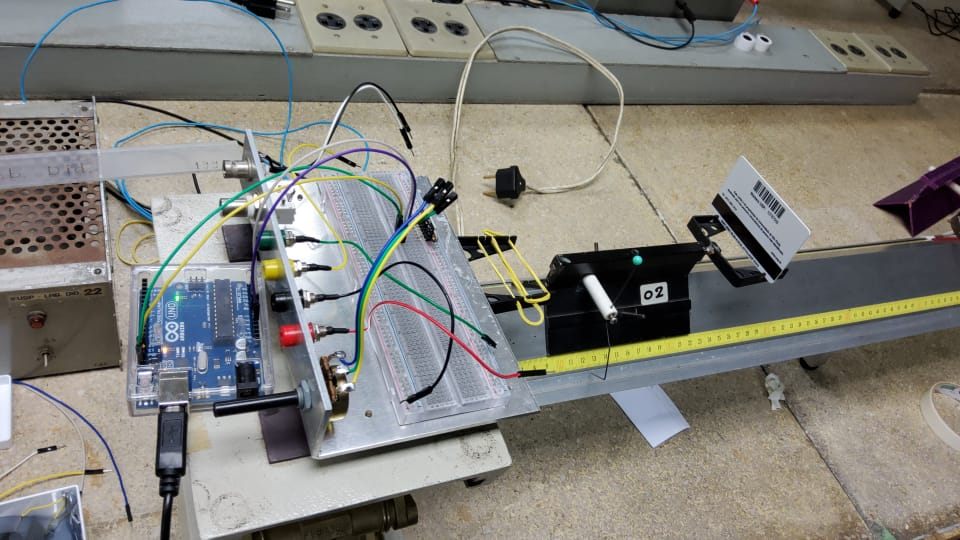
\includegraphics[scale=0.24]{06810750-c706-4d4c-a97f-17cbf277e8f1.jpg} 
\caption{Aparato experimental} 
\end{figure}

\begin{figure}[H] 
\centering
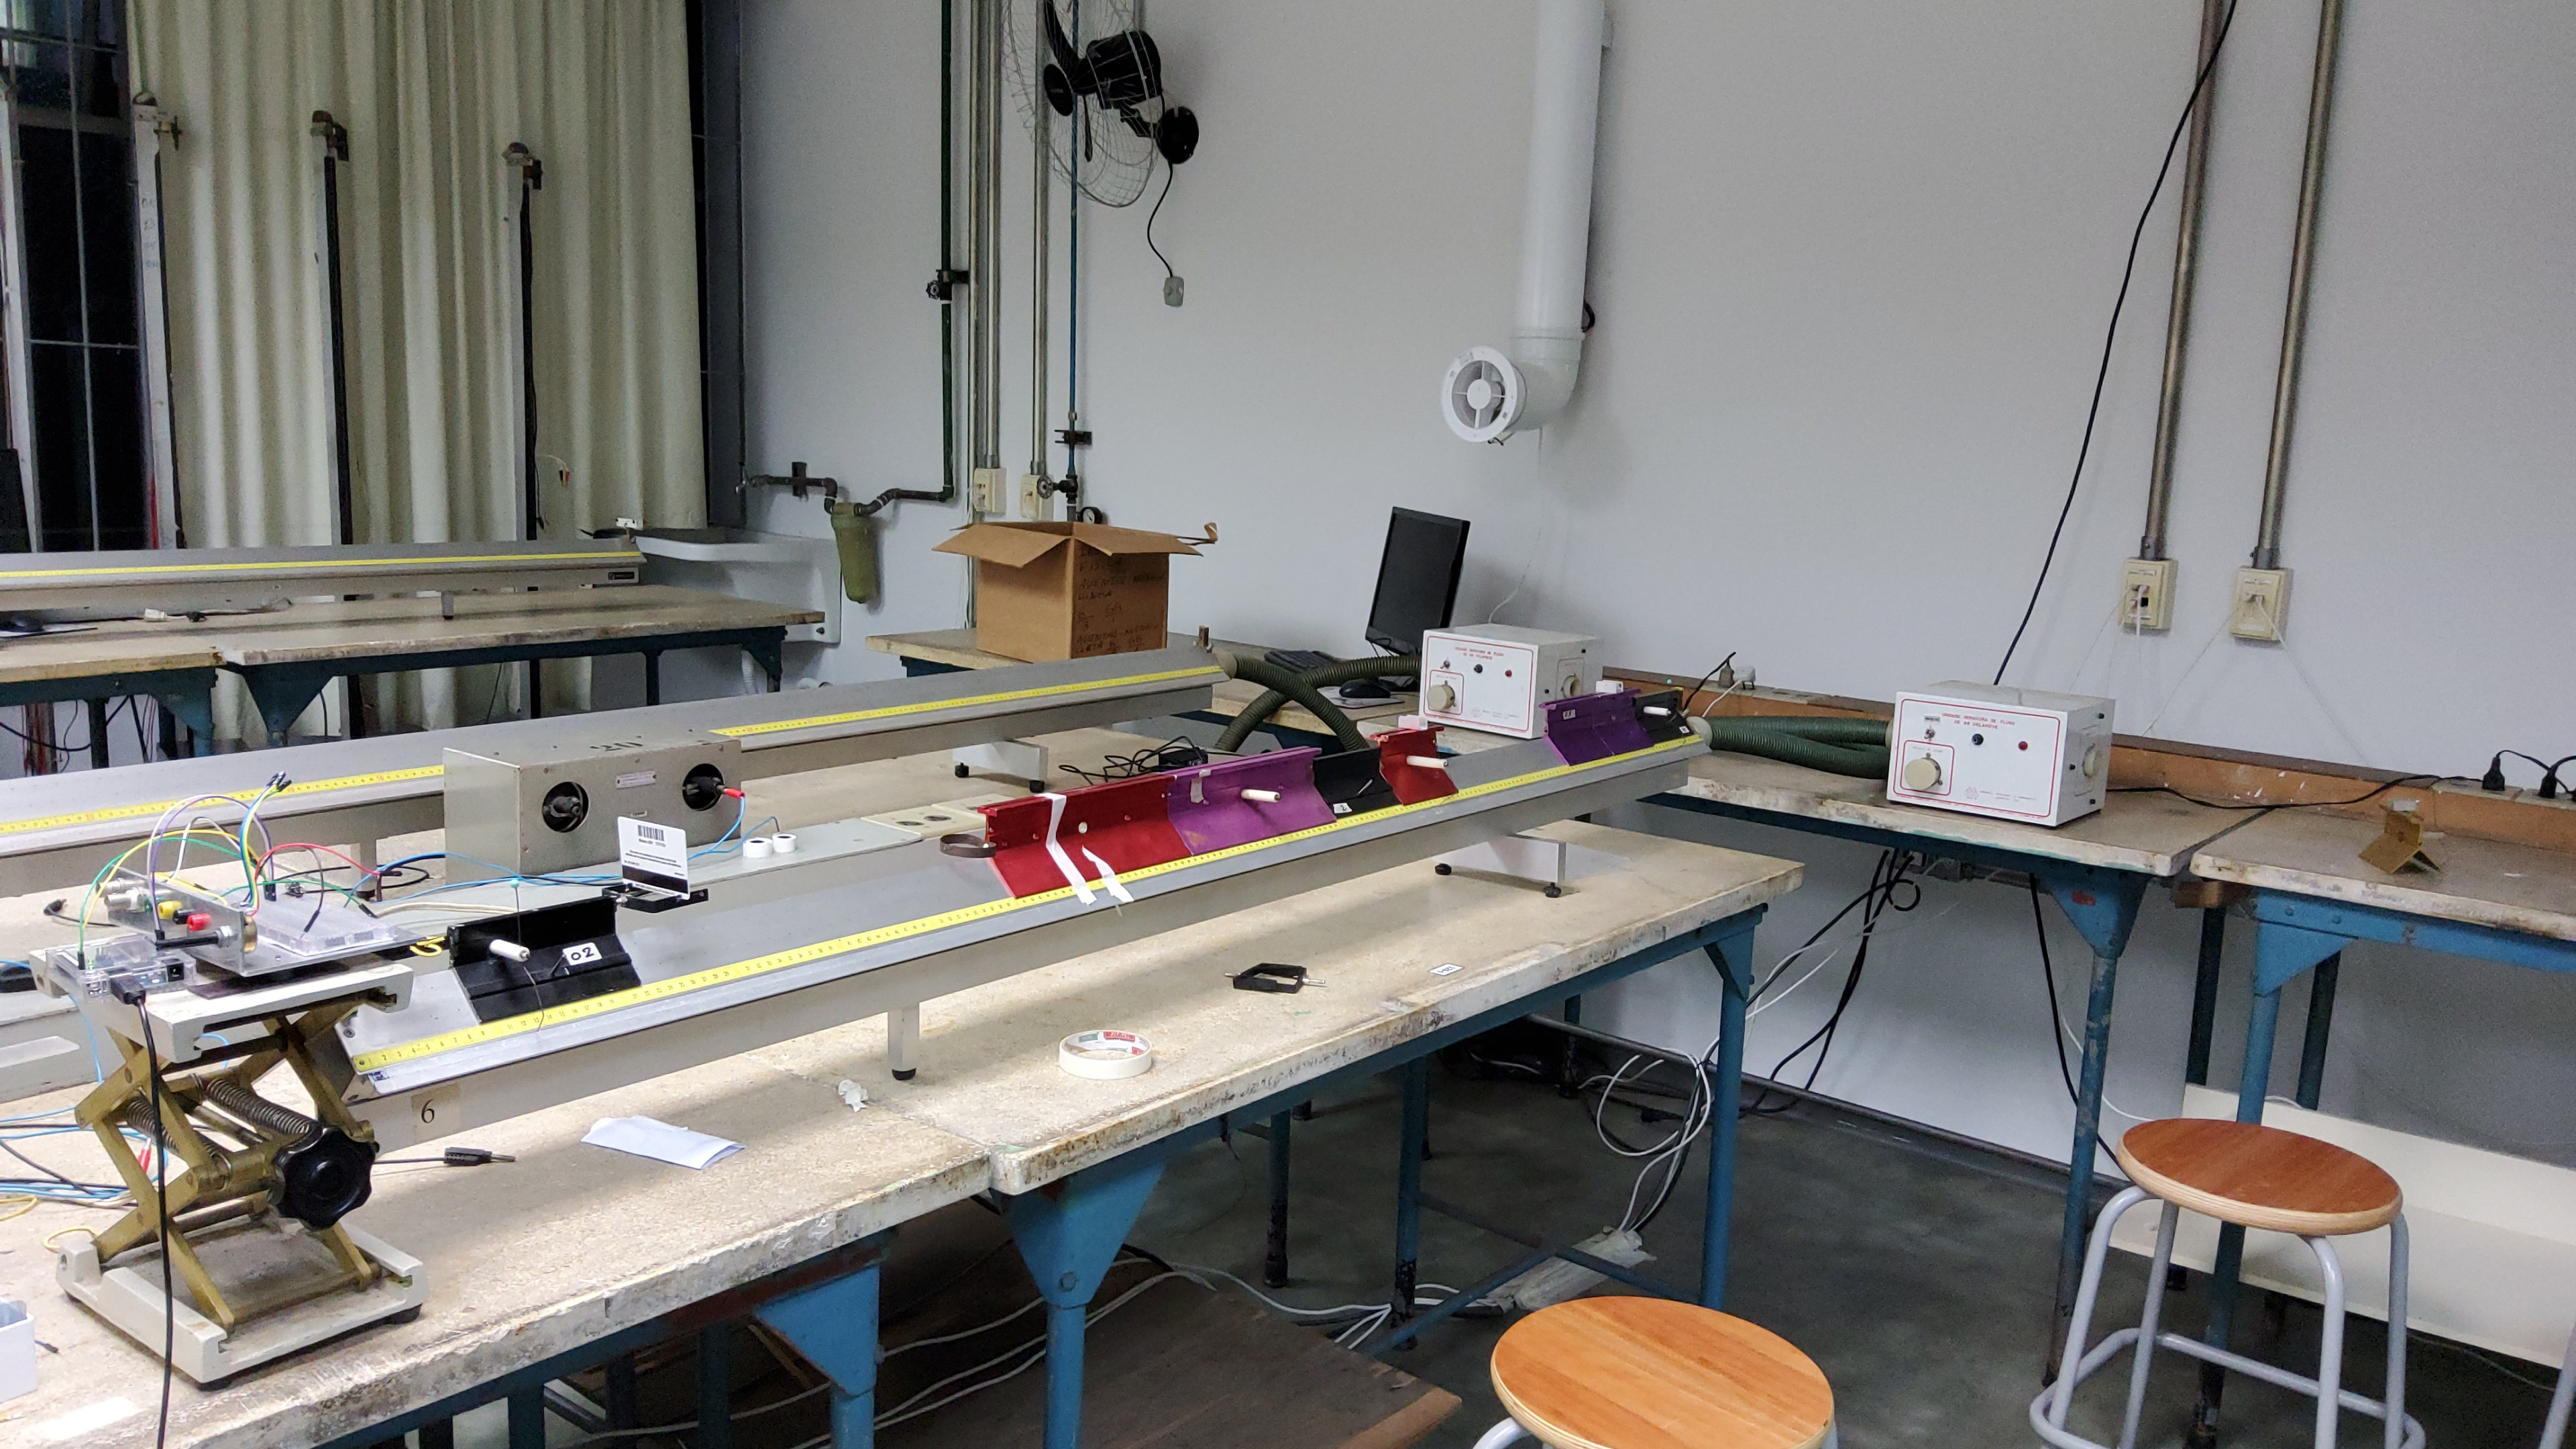
\includegraphics[scale=0.06]{IMG-20221206-WA0027.jpeg} 
\caption{Aparato experimental.} 
\end{figure}

\begin{figure}[H] 
\centering
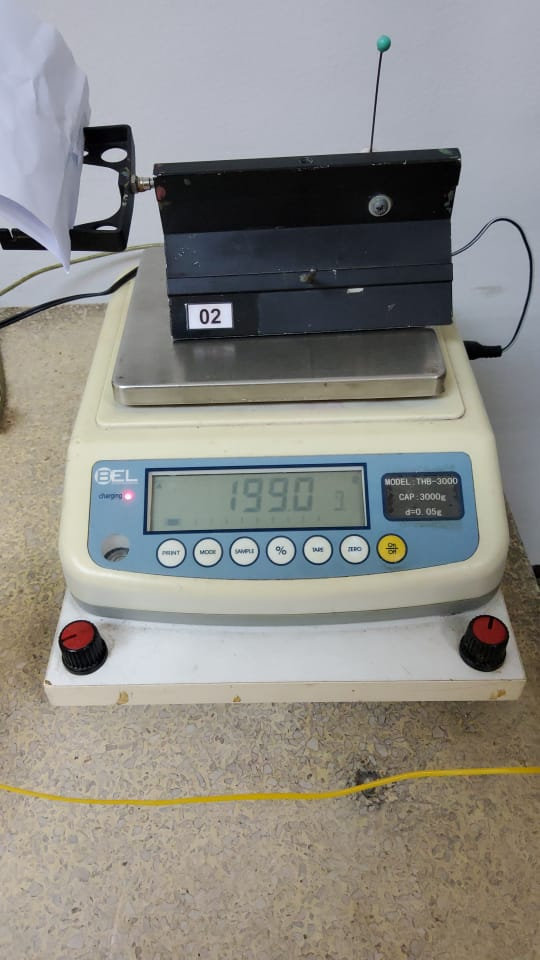
\includegraphics[scale=0.18]{1a4c4a09-f01b-4def-b72b-968d90990223.jpg} 
\caption{Aparato experimental.} 
\end{figure}

\begin{figure}[H] 
\centering
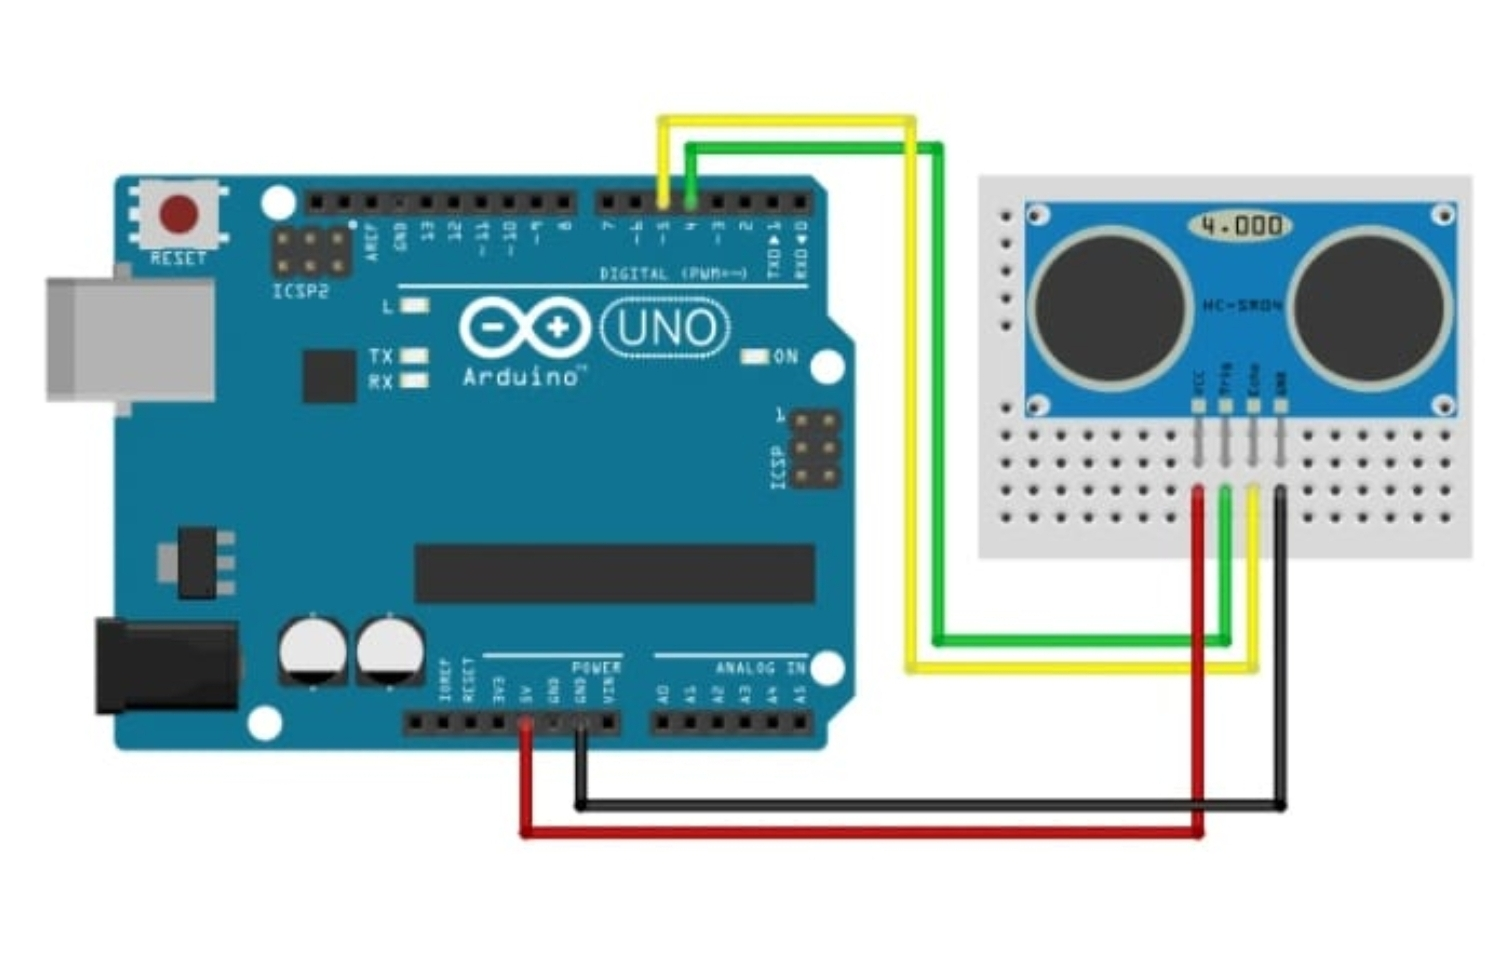
\includegraphics[scale=0.16]{circuito1.jpg} 
\caption{Circuito ultrassom} 
\end{figure}

\begin{figure}[H] 
\centering
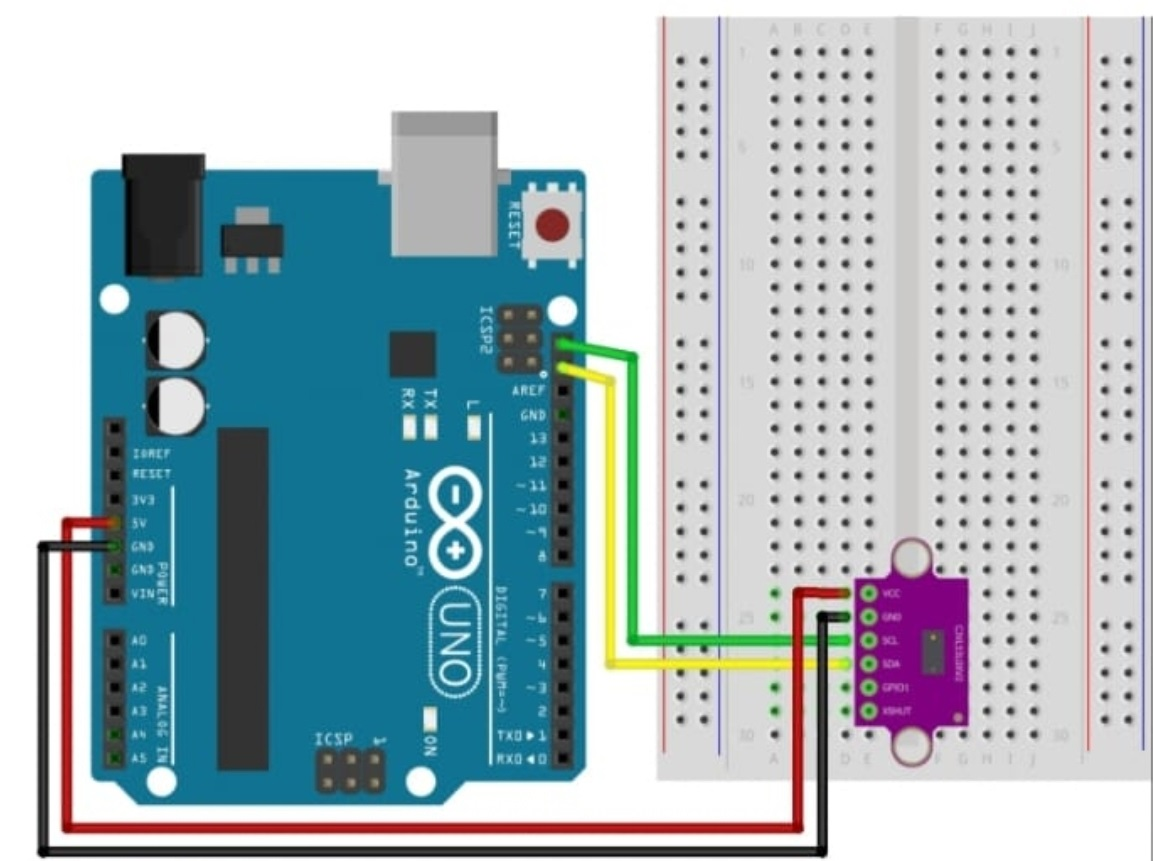
\includegraphics[scale=0.24]{circuito2.jpg} 
\caption{Circuito infravermelho} 
\end{figure}

\section{Orçamento}

Abaixo encontram-se os preços dos materiais utilizados para o experimento:

\begin{itemize}
    \item Trilho de ar: R\$ 6.461,41
    \item Protoboard: R\$ 15,00
    \item Sensor Ultrassonico: R\$ 23,00
    \item Sensor Lidar: R\$23,00
    \item Balança digital: R\$60,00
\end{itemize}

\begin{thebibliography}{1}

\bibitem[1]{Ultrassom}Como conectar o Sensor Ultrassônico HC-SR04 ao Arduino, https://www.filipeflop.com/blog/sensor-ultrassonico-hc-sr04-ao-arduino/, Data de acesso: 07/12/2022.

\bibitem[2]{Lidar}Radar with LiDAR sensor MIT, https://create.arduino.cc/projecthub/maksym-buryak/radar-with-lidar-sensor-877695, Data de acesso: 07/12/2022.

\end{thebibliography}

\end{multicols}
\end{document}